% Options for packages loaded elsewhere
\PassOptionsToPackage{unicode}{hyperref}
\PassOptionsToPackage{hyphens}{url}
\PassOptionsToPackage{dvipsnames,svgnames,x11names}{xcolor}
%
\documentclass[
  letterpaper,
  DIV=11,
  numbers=noendperiod]{scrreprt}

\usepackage{amsmath,amssymb}
\usepackage{lmodern}
\usepackage{iftex}
\ifPDFTeX
  \usepackage[T1]{fontenc}
  \usepackage[utf8]{inputenc}
  \usepackage{textcomp} % provide euro and other symbols
\else % if luatex or xetex
  \usepackage{unicode-math}
  \defaultfontfeatures{Scale=MatchLowercase}
  \defaultfontfeatures[\rmfamily]{Ligatures=TeX,Scale=1}
\fi
% Use upquote if available, for straight quotes in verbatim environments
\IfFileExists{upquote.sty}{\usepackage{upquote}}{}
\IfFileExists{microtype.sty}{% use microtype if available
  \usepackage[]{microtype}
  \UseMicrotypeSet[protrusion]{basicmath} % disable protrusion for tt fonts
}{}
\makeatletter
\@ifundefined{KOMAClassName}{% if non-KOMA class
  \IfFileExists{parskip.sty}{%
    \usepackage{parskip}
  }{% else
    \setlength{\parindent}{0pt}
    \setlength{\parskip}{6pt plus 2pt minus 1pt}}
}{% if KOMA class
  \KOMAoptions{parskip=half}}
\makeatother
\usepackage{xcolor}
\setlength{\emergencystretch}{3em} % prevent overfull lines
\setcounter{secnumdepth}{5}
% Make \paragraph and \subparagraph free-standing
\ifx\paragraph\undefined\else
  \let\oldparagraph\paragraph
  \renewcommand{\paragraph}[1]{\oldparagraph{#1}\mbox{}}
\fi
\ifx\subparagraph\undefined\else
  \let\oldsubparagraph\subparagraph
  \renewcommand{\subparagraph}[1]{\oldsubparagraph{#1}\mbox{}}
\fi


\providecommand{\tightlist}{%
  \setlength{\itemsep}{0pt}\setlength{\parskip}{0pt}}\usepackage{longtable,booktabs,array}
\usepackage{calc} % for calculating minipage widths
% Correct order of tables after \paragraph or \subparagraph
\usepackage{etoolbox}
\makeatletter
\patchcmd\longtable{\par}{\if@noskipsec\mbox{}\fi\par}{}{}
\makeatother
% Allow footnotes in longtable head/foot
\IfFileExists{footnotehyper.sty}{\usepackage{footnotehyper}}{\usepackage{footnote}}
\makesavenoteenv{longtable}
\usepackage{graphicx}
\makeatletter
\def\maxwidth{\ifdim\Gin@nat@width>\linewidth\linewidth\else\Gin@nat@width\fi}
\def\maxheight{\ifdim\Gin@nat@height>\textheight\textheight\else\Gin@nat@height\fi}
\makeatother
% Scale images if necessary, so that they will not overflow the page
% margins by default, and it is still possible to overwrite the defaults
% using explicit options in \includegraphics[width, height, ...]{}
\setkeys{Gin}{width=\maxwidth,height=\maxheight,keepaspectratio}
% Set default figure placement to htbp
\makeatletter
\def\fps@figure{htbp}
\makeatother

\KOMAoption{captions}{tableheading}
\makeatletter
\makeatother
\makeatletter
\@ifpackageloaded{bookmark}{}{\usepackage{bookmark}}
\makeatother
\makeatletter
\@ifpackageloaded{caption}{}{\usepackage{caption}}
\AtBeginDocument{%
\ifdefined\contentsname
  \renewcommand*\contentsname{Table of contents}
\else
  \newcommand\contentsname{Table of contents}
\fi
\ifdefined\listfigurename
  \renewcommand*\listfigurename{List of Figures}
\else
  \newcommand\listfigurename{List of Figures}
\fi
\ifdefined\listtablename
  \renewcommand*\listtablename{List of Tables}
\else
  \newcommand\listtablename{List of Tables}
\fi
\ifdefined\figurename
  \renewcommand*\figurename{Figure}
\else
  \newcommand\figurename{Figure}
\fi
\ifdefined\tablename
  \renewcommand*\tablename{Table}
\else
  \newcommand\tablename{Table}
\fi
}
\@ifpackageloaded{float}{}{\usepackage{float}}
\floatstyle{ruled}
\@ifundefined{c@chapter}{\newfloat{codelisting}{h}{lop}}{\newfloat{codelisting}{h}{lop}[chapter]}
\floatname{codelisting}{Listing}
\newcommand*\listoflistings{\listof{codelisting}{List of Listings}}
\makeatother
\makeatletter
\@ifpackageloaded{caption}{}{\usepackage{caption}}
\@ifpackageloaded{subcaption}{}{\usepackage{subcaption}}
\makeatother
\makeatletter
\@ifpackageloaded{tcolorbox}{}{\usepackage[many]{tcolorbox}}
\makeatother
\makeatletter
\@ifundefined{shadecolor}{\definecolor{shadecolor}{rgb}{.97, .97, .97}}
\makeatother
\makeatletter
\makeatother
\ifLuaTeX
\usepackage[bidi=basic]{babel}
\else
\usepackage[bidi=default]{babel}
\fi
\babelprovide[main,import]{american}
% get rid of language-specific shorthands (see #6817):
\let\LanguageShortHands\languageshorthands
\def\languageshorthands#1{}
\ifLuaTeX
  \usepackage{selnolig}  % disable illegal ligatures
\fi
\IfFileExists{bookmark.sty}{\usepackage{bookmark}}{\usepackage{hyperref}}
\IfFileExists{xurl.sty}{\usepackage{xurl}}{} % add URL line breaks if available
\urlstyle{same} % disable monospaced font for URLs
\hypersetup{
  pdftitle={RKWard - Manual},
  pdflang={en-US},
  colorlinks=true,
  linkcolor={blue},
  filecolor={Maroon},
  citecolor={Blue},
  urlcolor={Blue},
  pdfcreator={LaTeX via pandoc}}

\title{RKWard - Manual}
\author{}
\date{8/26/23}

\begin{document}
\maketitle
\ifdefined\Shaded\renewenvironment{Shaded}{\begin{tcolorbox}[breakable, enhanced, borderline west={3pt}{0pt}{shadecolor}, sharp corners, interior hidden, boxrule=0pt, frame hidden]}{\end{tcolorbox}}\fi

\renewcommand*\contentsname{Table of contents}
{
\hypersetup{linkcolor=}
\setcounter{tocdepth}{2}
\tableofcontents
}
\bookmarksetup{startatroot}

\hypertarget{welcome}{%
\chapter*{Welcome}\label{welcome}}
\addcontentsline{toc}{chapter}{Welcome}

\markboth{Welcome}{Welcome}

This is a \textbf{RKWard} book manual. \textbf{RKWard} is an easy to use
and easily extensible \textbf{IDE/GUI for R}.

\hypertarget{versions}{%
\section*{Versions}\label{versions}}
\addcontentsline{toc}{section}{Versions}

\markright{Versions}

The \textbf{RKWard} version used in this book is \textbf{0.7.5 - 24 Oct
2022}.

The R Version is: 4.2.0

Windows 10 x64 (build 19045)

x86\_64-w64-mingw32/x64 (64-bit)

\begin{center}\rule{0.5\linewidth}{0.5pt}\end{center}

Last update: 08/26/2023 - 12:38:42 -03

\bookmarksetup{startatroot}

\hypertarget{about-rkward}{%
\chapter{About RKWard}\label{about-rkward}}

\hypertarget{rkward-mission-statement}{%
\section{\texorpdfstring{\href{https://rkward.kde.org/RKWard_Overview.html}{RKWard
Mission
statement}}{RKWard Mission statement}}\label{rkward-mission-statement}}

\textbf{RKWard} is meant to become an easy to use, transparent frontend
to the \href{http://r-project.org/}{R-language}, a very powerful, yet
hard-to-get-into scripting-language with a strong focus on statistic
functions. It will not only provide a convenient user-interface,
however, but also take care of seamless integration with an
office-suite. Practical statistics is not just about calculating, after
all, but also about documenting and ultimately publishing the results.

\textbf{RKWard} then is (will be) something like a free replacement for
commercial statistical packages. In addition to ease of use, three
aspects are particularily important:

\begin{itemize}
\item
  It will be a transparent interface to the underlying R-language. That
  is, it will not hide the powerful syntax, but merely provide a
  convenient way, in which both newbies and R-experts can accomplish
  most of their tasks. A GUI can never provide an interface to the whole
  power of a language like R. In some cases users will want to tweak
  some functions to their particular needs and esp.~to automate some
  tasks. By making the ``inner workings'' visible to the user,
  \textbf{RKWard} will make it easy for the user to see where and how to
  use R-syntax to accomplish their goals.
\item
  For the output, \textbf{RKWard} strives to separate content and design
  to a high degree. It will not try to design its own tables/graphs,
  etc, which have to be converted to the style used in the rest of a
  publication by hand. Currently \textbf{RKWard} uses HTML for its
  output. Using appropriate style definitions reformatting this output
  to match the rest of the publication will be easily doable. In future
  releases \textbf{RKWard} will even seek stronger integration with
  existing office suites.
\item
  It relies on a language, that is not only very powerful, but also
  extensible, and for which dozens of extensions already exist.
\end{itemize}

\textbf{And of course, it is free (as in free speech).}

\textbf{Current status}

Perhaps the best way to get an impression of the current state of
\textbf{RKWard} (other than installing and trying it) is to have a look
at the Screenshots. A status page focused on the internal components is
here.

\textbf{In summary}:

\textbf{RKWard} currently offers a lot of useful features for developing
R code. This functionality makes \textbf{RKWard} highly useful as an IDE
for R experts, today. The number of graphical dialogs to give access to
statistical functions is still rather limited. Users coming from
competing graphical statistics suites will find a lot is still missing,
but possibly the functionality you need most is already implemented in
the growing number of plugins. Why don't you give it a try to find out?
It is also possible to add your own dialogs as plugins (see Developer
Information\#Plugin developers). As far as office integration is
concerned, \textbf{RKWard} still has a long way to go. However, results
are stored to in HTML format, however, making it easy to copy-and-paste
or import them into text-processing or other office tools.

\hypertarget{about-rkward-1}{%
\section{\texorpdfstring{About
\textbf{RKWard}}{About RKWard}}\label{about-rkward-1}}

\textbf{RKWard} is developed by a community of volunteers.

\begin{figure}

{\centering 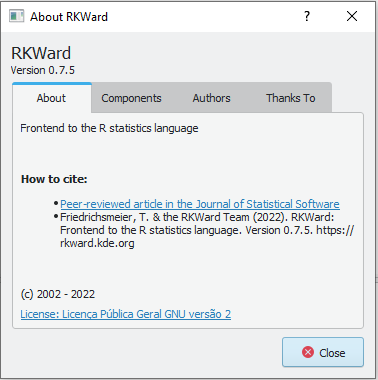
\includegraphics{./images/about_rkward.png}

}

\caption{About \textbf{RKWard}}

\end{figure}

\begin{figure}

{\centering 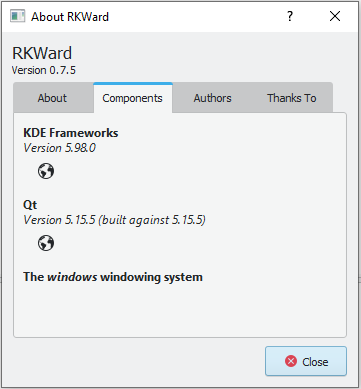
\includegraphics{./images/about_components.png}

}

\caption{\textbf{RKWard} Components}

\end{figure}

\begin{figure}

{\centering 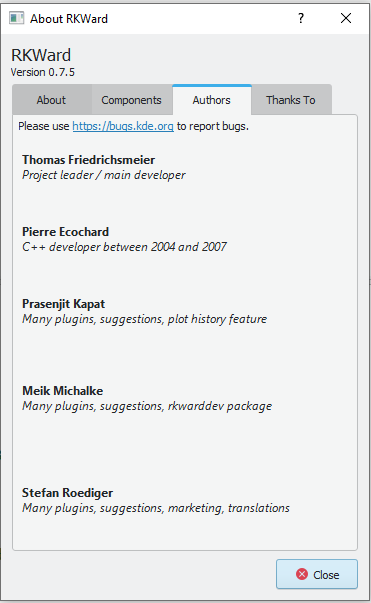
\includegraphics{./images/about_authors.png}

}

\caption{\textbf{RKWard} Authors}

\end{figure}

\hypertarget{rkward-0.7.5---24-oct-2022}{%
\section{\texorpdfstring{\textbf{RKWard} 0.7.5 - 24 Oct
2022}{RKWard 0.7.5 - 24 Oct 2022}}\label{rkward-0.7.5---24-oct-2022}}

A new release, \textbf{RKWard} 0.7.5, is available for download, today.

The most visible changes are the inclusion of many new and improved code
snippets, and option to restart the R backend without leaving RKWard
(this can be very useful when trying to make sure that a script is fully
reproducible), and various improvements to code completion in scripts
and the R Console.

As usual, we're looking forward to your feedback suggestions, and
contributions!

The changes in detail:

\textbf{New features and improvements}

\begin{itemize}
\tightlist
\item
  Added: Partial completions (Tab-key) consider completion candidates
  from all visible completion groups
\item
  Added: R's dynamic completions (importantly for ``:::'', ``?'', and
  ``@'') are merged into the already provided completions
\item
  Added: Add option to offer code completion/hinting in all file types
  not just R scripts (e.g.~in .Rmd files)
\item
  Changed default behavior (new installations, only): Up/down without
  alt navigate completion items if visible in console/editor
\item
  Added: Provide tooltips on symbols in scripts and R console
\item
  Added: Many new basic and advanced R, R Markdown and LaTeX snippets,
  including complete R Markdown templates
\item
  Added: Allow to select search provider, when searching for a term
  online
\item
  Added: Allow to restart R backend (e.g.~for testing that scripts or
  packages will work in a fresh session)
\item
  Changed: Actions to restart the R backend, interrupt all commands and
  configure the R backend arranged in a hmburger menu
\item
  Added: Crosstabs N to N: Simplify labels, add option to control table
  layout
\item
  Added: Change mechanism for detection of object changes
\end{itemize}

\textbf{Bug fixes}

\begin{itemize}
\tightlist
\item
  Fixed: Backend failed to start when installed in a path with spaces on
  Windows volumes without 8.3 support
\item
  Fixed: Trying to restart backend could cause a hang, on Windows
\item
  Fixed: In corner cases, cancelling commands could lead to a lockup
\item
  Fixed: IRT Cronbach's Alpha did not work for subsets, if the
  data.frame name contains dots
\item
  Fixed: Action to remove several rows in data editor, simultaneously,
  always remained disabled
\item
  Fixed: Workspace browser would not always show change, immediately,
  when object type changes
\item
  Fixed: Crash when using the ``Git blame'' kate plugin
\item
  Fixed: Problem installing R support package in some configurations
\item
  Fixed: Menubar would disapper after opening script editor, in some
  configurations
\item
  Fixed: Very long error messages during R markdown preview could cause
  the preview window to become too wide
\item
  Fixed: Expresssions spanning several lines would not be shown,
  correctly, in ``R Console''-mode script preview
\item
  Fixed: Fix focus problems, and better efficiency for data previews (as
  used in data import dialogs)
\item
  Fixed: Excel import plugin failed to accept file name
\item
  Fixed: Fix zooming help/output pages with Ctrl+scroll wheel, when
  compiled with QWebEngine
\item
  Fixed: Fix problem handling rkward:// links from dialogs on some
  sytems
\item
  Fixed: Fix object name completion for (irregular) names starting with
  numbers or underscores
\end{itemize}

\begin{center}\rule{0.5\linewidth}{0.5pt}\end{center}

Last update: 08/26/2023 - 12:38:01 -03

\bookmarksetup{startatroot}

\hypertarget{screenshots}{%
\chapter{Screenshots}\label{screenshots}}

\href{https://rkward.kde.org/Screenshots.html}{Screenshots}

\hypertarget{main-window}{%
\section{Main Window}\label{main-window}}

The main application window with a dashboard of recent files and common
tasks. At the left and there are several buttons to expand / collapse
tool windows (RKWard 0.7.5).

\begin{figure}

{\centering 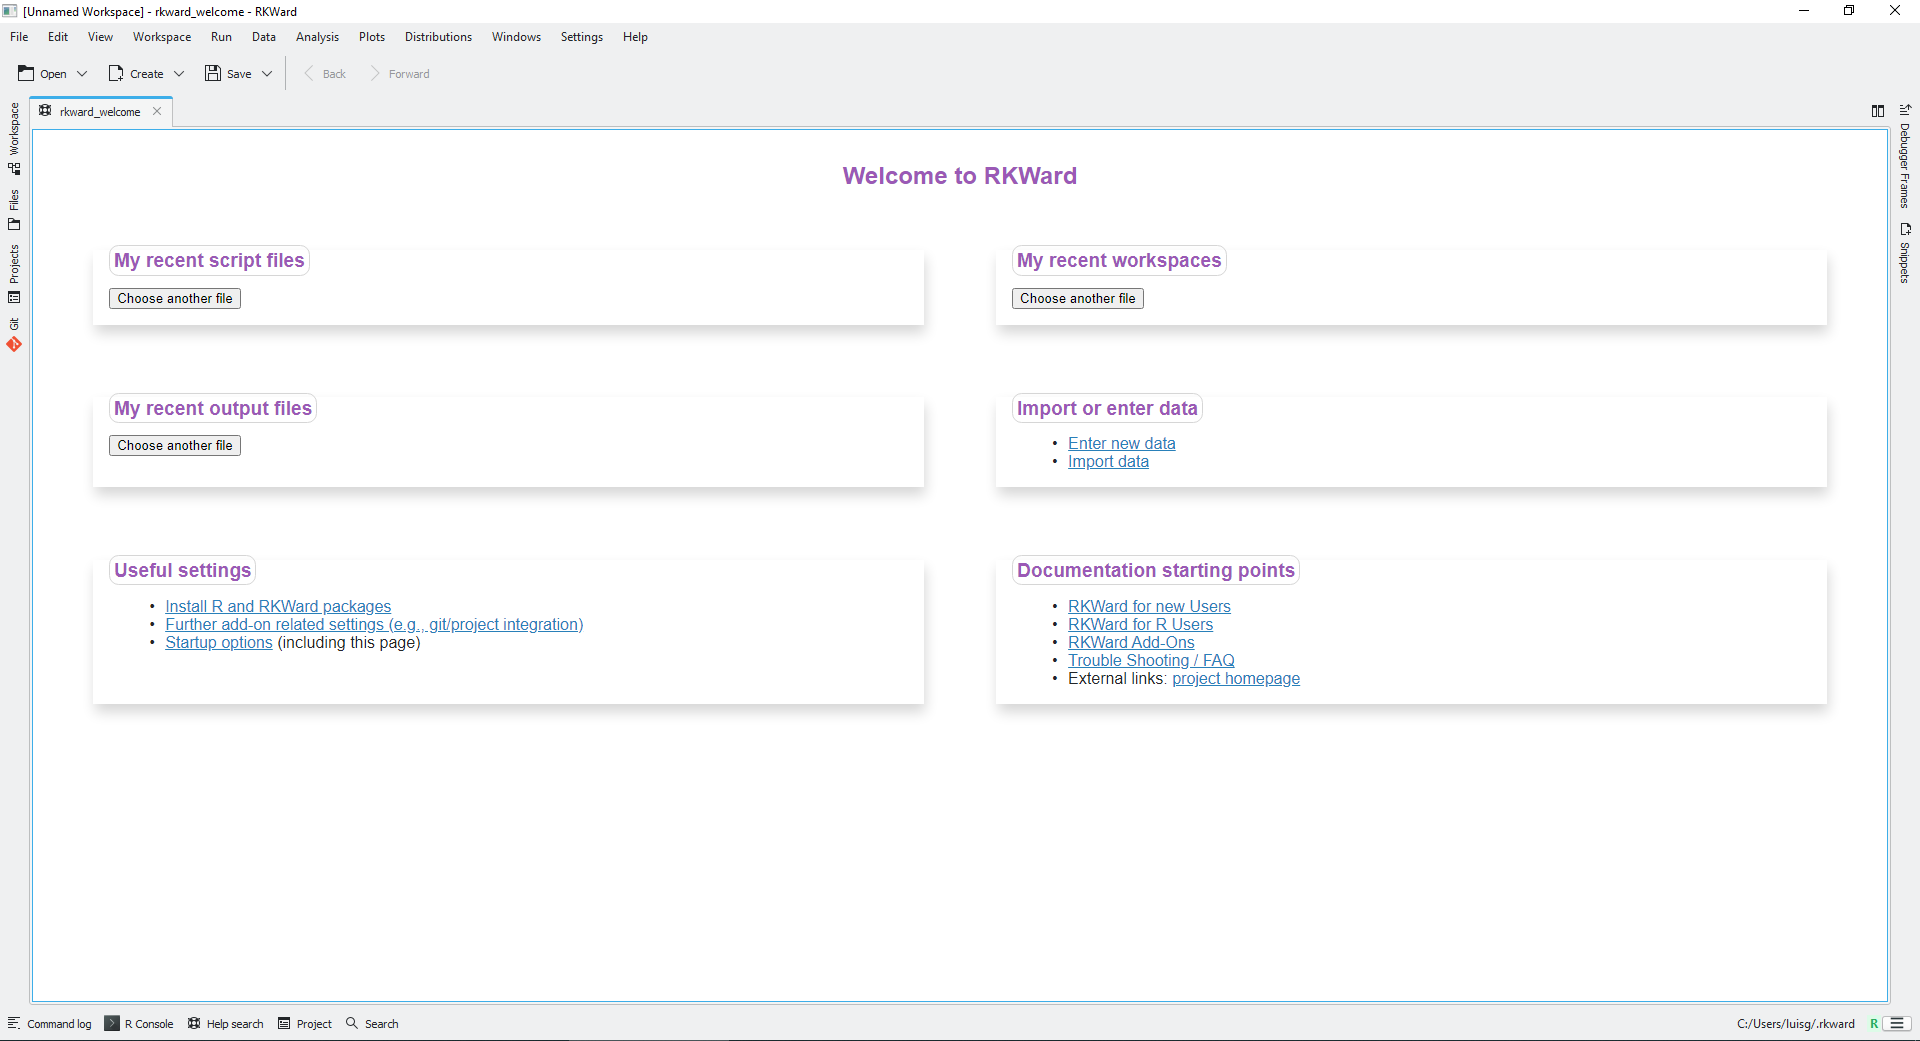
\includegraphics{./images/main_window.png}

}

\caption{Main Window}

\end{figure}

The application window with the Workspace Browser, Data Editor, File
Browser, and RConsole tabs expanded and attached to the main window.

\begin{figure}

{\centering 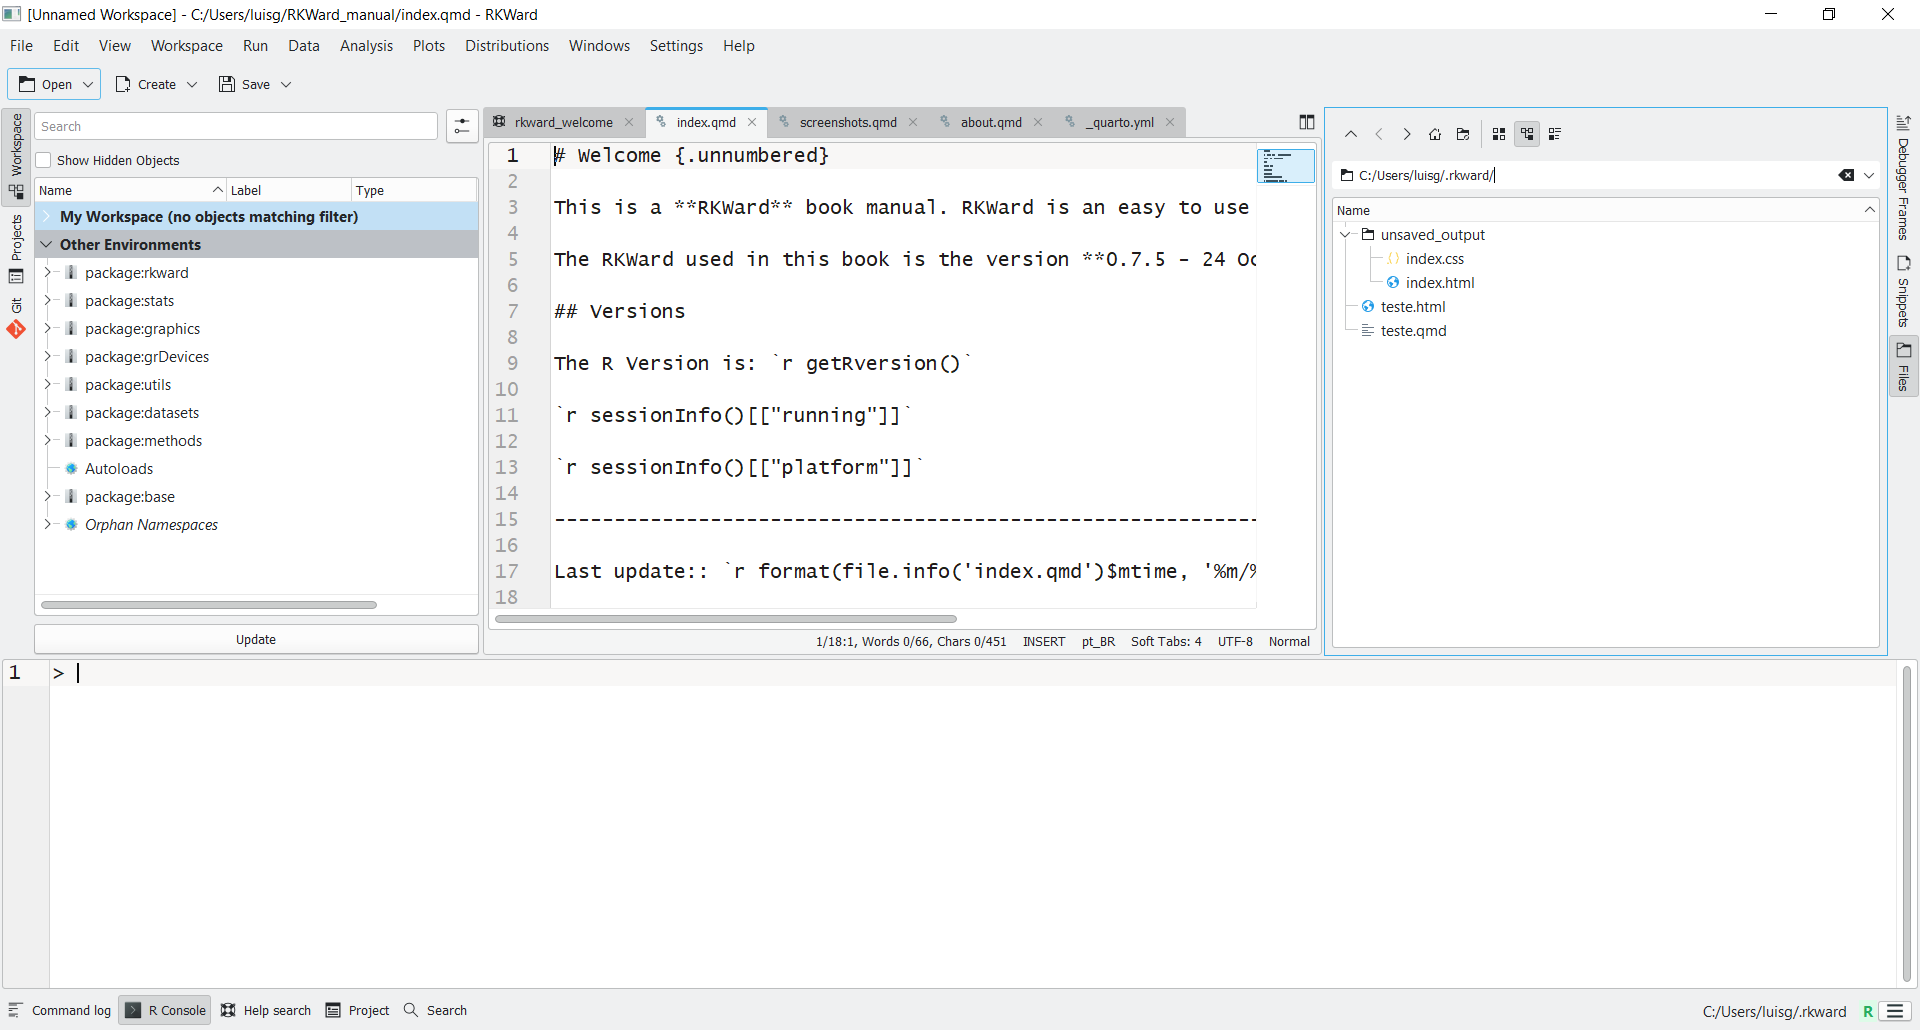
\includegraphics{./images/main_tabs.png}

}

\caption{Tabs}

\end{figure}

The placement can be re-arranged, and each individual window can also be
detached as a separate top level window (Windows \textgreater{} Detach).

\begin{figure}

{\centering 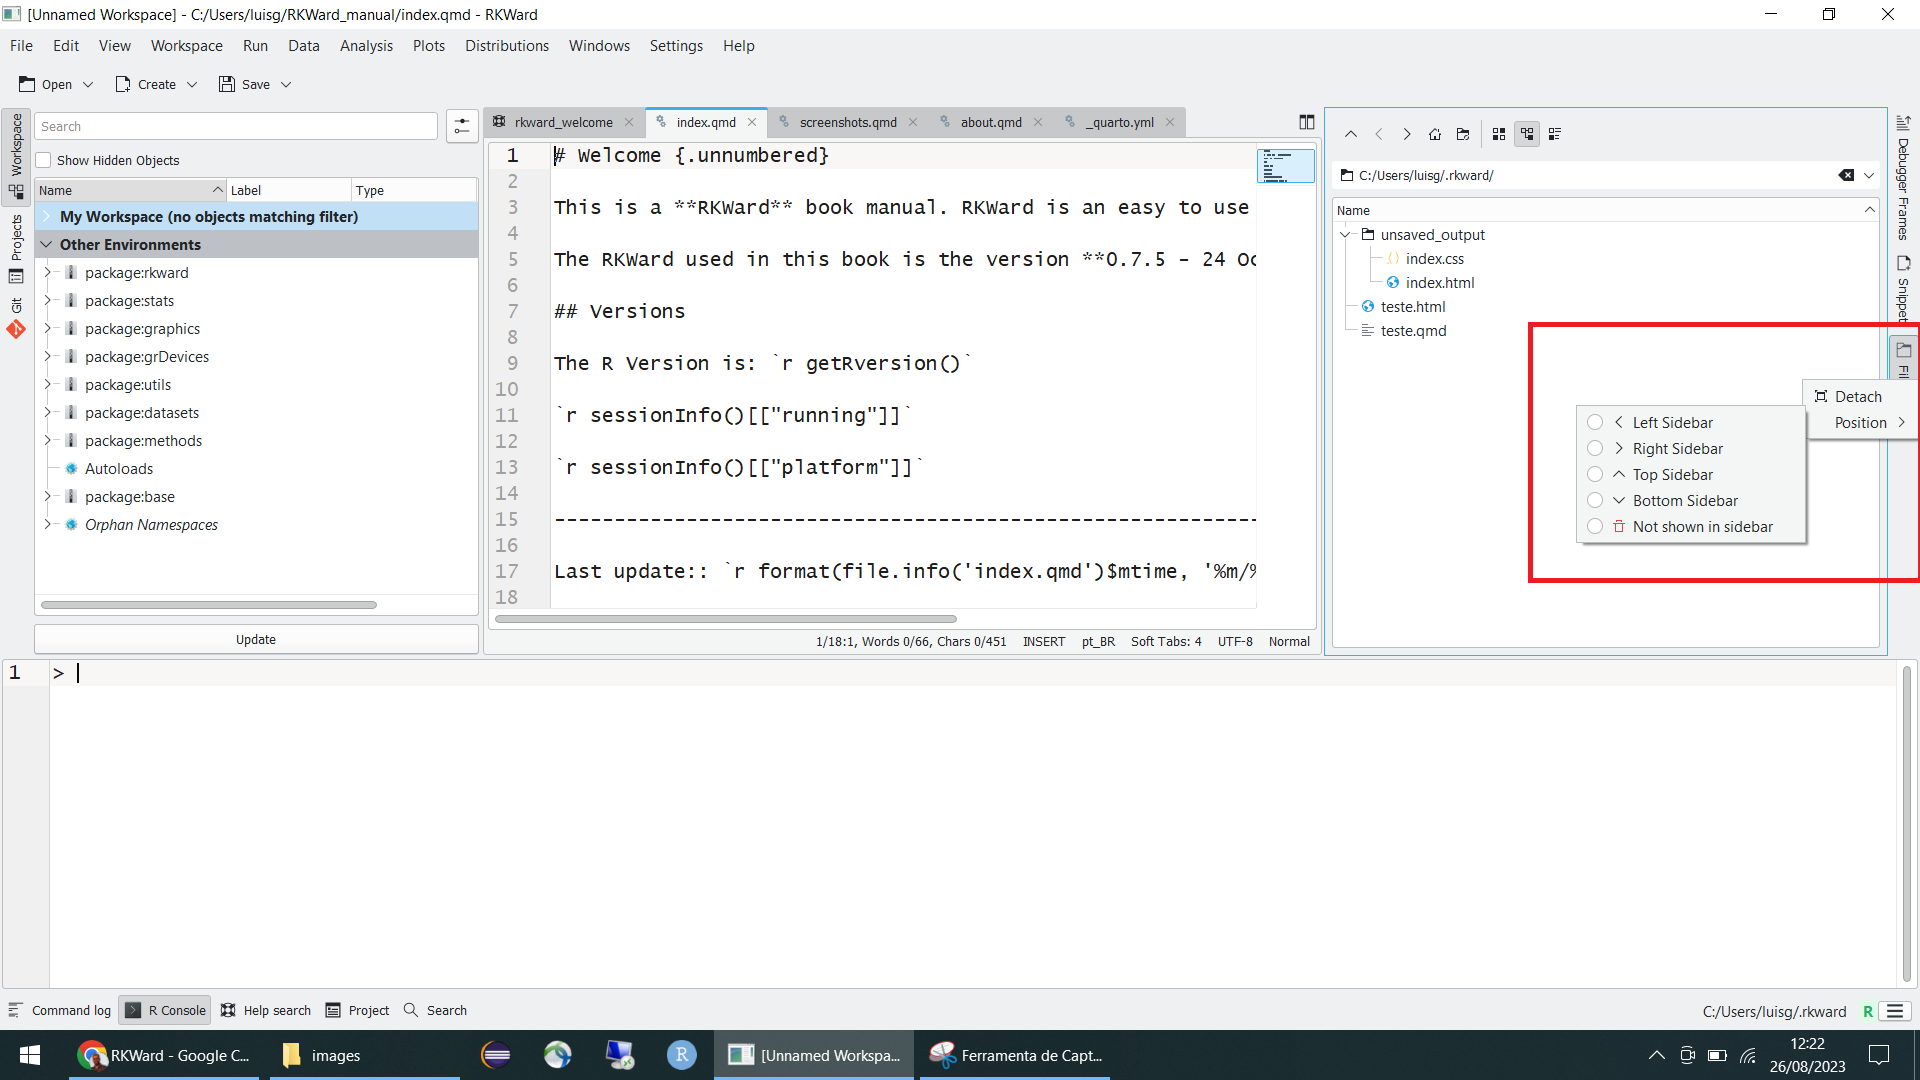
\includegraphics{./images/main_tabs_position.png}

}

\caption{Tabs Position}

\end{figure}

\begin{center}\rule{0.5\linewidth}{0.5pt}\end{center}

Last update: 08/26/2023 - 12:37:56 -03

\bookmarksetup{startatroot}

\hypertarget{menu-file}{%
\chapter{Menu file}\label{menu-file}}

\begin{figure}

{\centering 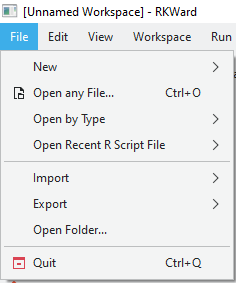
\includegraphics{./images/menu_file/menu_file.png}

}

\caption{Menu File}

\end{figure}

\begin{figure}

{\centering \includegraphics{./images/menu_file/menu_new.png}

}

\caption{Menu File}

\end{figure}

\begin{figure}

{\centering 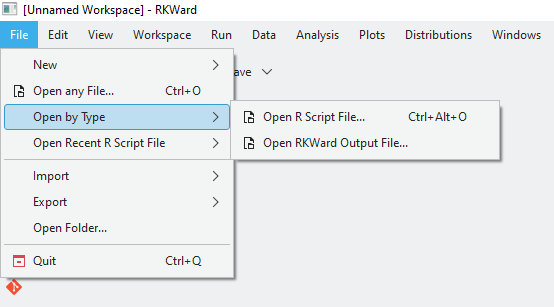
\includegraphics{./images/menu_file/menu_file_open_type.png}

}

\caption{Menu File}

\end{figure}

\begin{figure}

{\centering 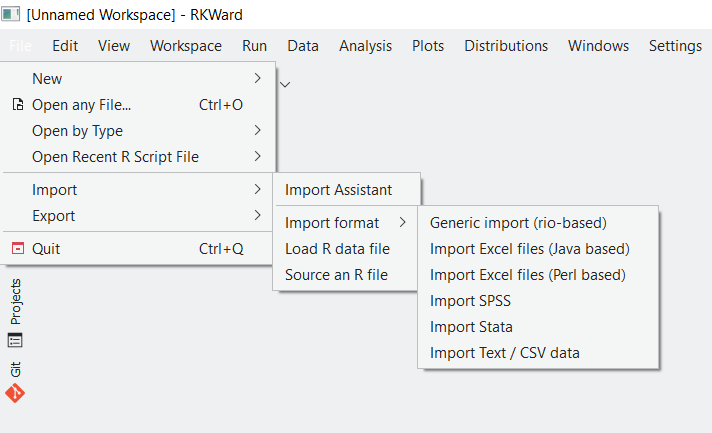
\includegraphics{./images/menu_file/menu_file_import_format.png}

}

\caption{Menu File}

\end{figure}

\begin{figure}

{\centering 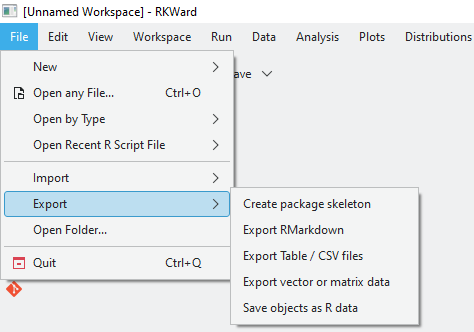
\includegraphics{./images/menu_file/menu_file_export.png}

}

\caption{Menu File}

\end{figure}

\begin{figure}

{\centering 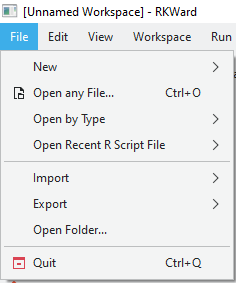
\includegraphics{./images/menu_file/menu_file.png}

}

\caption{Menu File}

\end{figure}

\begin{figure}

{\centering 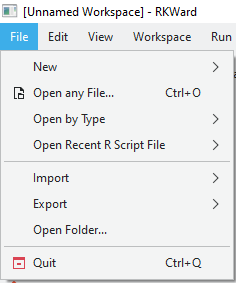
\includegraphics{./images/menu_file/menu_file.png}

}

\caption{Menu File}

\end{figure}

\begin{center}\rule{0.5\linewidth}{0.5pt}\end{center}

Last update: 08/26/2023 - 13:56:47 -03



\end{document}
